\documentclass{article}
\usepackage{amsmath,amssymb}
\usepackage{tikz}
\usetikzlibrary{arrows.meta,positioning,calc,shapes.geometric}
\pagestyle{empty}
\begin{document}
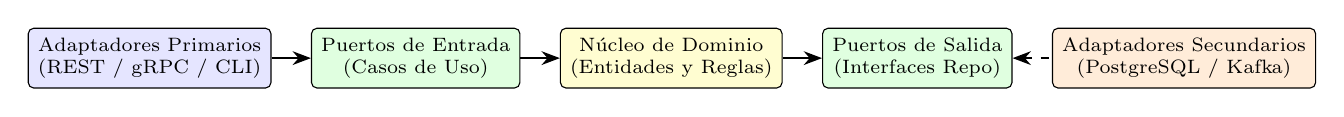
\begin{tikzpicture}
\tikzset{node distance=0.5cm, every node/.style={font=\scriptsize, draw, rounded corners=2pt, align=center, inner sep=3.5pt}}
\node (in) [fill=blue!10] {Adaptadores Primarios\\(REST / gRPC / CLI)};
\node (usecase) [right=of in, fill=green!12] {Puertos de Entrada\\(Casos de Uso)};
\node (domain) [right=of usecase, fill=yellow!18] {Núcleo de Dominio\\(Entidades y Reglas)};
\node (portout) [right=of domain, fill=green!12] {Puertos de Salida\\(Interfaces Repo)};
\node (out) [right=of portout, fill=orange!15] {Adaptadores Secundarios\\(PostgreSQL / Kafka)};
\draw[-Stealth, thick] (in) -- (usecase);
\draw[-Stealth, thick] (usecase) -- (domain);
\draw[-Stealth, thick] (domain) -- (portout);
\draw[Stealth-, thick, dashed] (portout) -- (out);
\end{tikzpicture}
\end{document}
